In this project, the goal is to label all faces in the given image as mask/no mask. For example:

\begin{figure}[H]
    \centering
    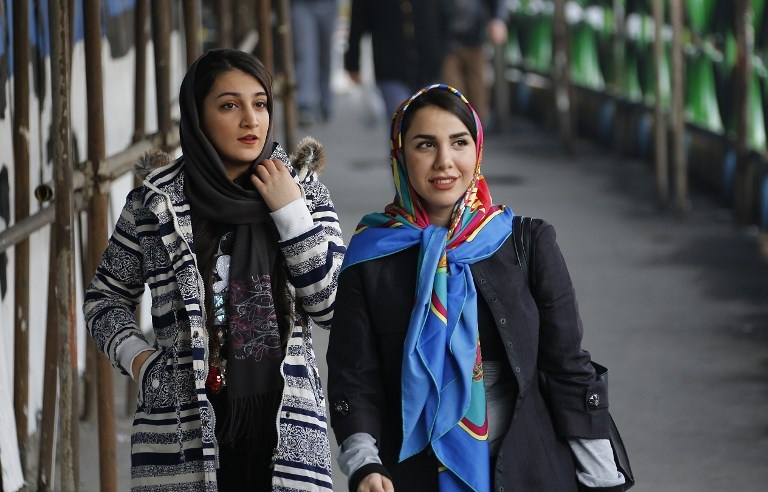
\includegraphics[width=0.7\textwidth]{Orig.jpeg}
    \caption{Original Image}
    \label{fig:Orig}
\end{figure}

\begin{figure}[H]
    \centering
    
\includegraphics[width=0.3\textwidth]{Person1.jpg}
    \caption{First Image}
    \label{fig:First}
\end{figure}

\begin{figure}[H]
    \centering
    
\includegraphics[width=0.3\textwidth]{Person2.jpg}
    \caption{Second Image}
    \label{fig:Second}
\end{figure}

We'll need to determine which of these women is wearing a medical mask.

\subsection{Approach}
We are interested in labels
\begin{itemize}
    \item Face with mask
    \item Face without mask
\end{itemize}

We want to train a binary classifier to predict mask true or false for a given facial image.


The problem with this approach is that face detector might be less accurate on faces with masks on.

\subsection{The Solution}
We will train a model with three classes:
\begin{enumerate}
    \item Face with mask
    \item Face without mask
    \item Not a face
    \item Mask worn incorrectly (*will be hard to implement)
\end{enumerate}

and apply it “efficiently” to a larger input image.

\subsection{The Method}
\subsubsection{Train}
We'll have two models:
\begin{enumerate}
    \item Pre-trained Face Detector:

        Input: frame

	    Output: Cropped human face
    \item A model with three classes: masked, non-masked (equally distributed) \& non-face
\end{enumerate}


\subsubsection{Test}
\begin{itemize}
    \item Take an image or a Frame from a camera/video
    \item Determine if the object/s in the picture are human (using second model)
    \item Crop the object/s one by one (using first model), \& determine masked/non-masked (using second model)
\end{itemize}


